%
% Main document
% ===========================================================================
% This is part of the document "Project documentation template".
% Authors: brd3, kaa1
%

%---------------------------------------------------------------------------
\documentclass[
	a4paper,					% paper format
	10pt,							% fontsize
	twoside,					% double-sided
	openright,				% begin new chapter on right side
	notitlepage,			% use no standard title page
	parskip=half,			% set paragraph skip to half of a line
]{scrreprt}					% KOMA-script report
%---------------------------------------------------------------------------

\raggedbottom
\KOMAoptions{cleardoublepage=plain}			% Add header and footer on blank pages


% Load Standard Packages:
%---------------------------------------------------------------------------
\usepackage[standard-baselineskips]{cmbright}

\usepackage[english]{babel}										% english hyphenation
%\usepackage[latin1]{inputenc}  							% Unix/Linux - load extended character set (ISO 8859-1)
\usepackage[ansinew]{inputenc}  							% Windows - load extended character set (ISO 8859-1)
\usepackage[T1]{fontenc}											% hyphenation of words with �,� and �
\usepackage{textcomp}													% additional symbols
\usepackage{ae}																% better resolution of Type1-Fonts 
\usepackage{fancyhdr}													% simple manipulation of header and footer 
\usepackage{etoolbox}													% color manipulation of header and footer
\usepackage{graphicx}                      		% integration of images
\usepackage{float}														% floating objects
\usepackage{caption}													% for captions of figures and tables
\usepackage{booktabs}													% package for nicer tables
\usepackage{tocvsec2}													% provides means of controlling the sectional numbering
%---------------------------------------------------------------------------

% Load Math Packages
%---------------------------------------------------------------------------
\usepackage{amsmath}                    	   	% various features to facilitate writing math formulas
\usepackage{amsthm}                       	 	% enhanced version of latex's newtheorem
\usepackage{amsfonts}                      		% set of miscellaneous TeX fonts that augment the standard CM
\usepackage{amssymb}													% mathematical special characters
\usepackage{exscale}													% mathematical size corresponds to textsize
%---------------------------------------------------------------------------

% Package to facilitate placement of boxes at absolute positions
%---------------------------------------------------------------------------
\usepackage[absolute]{textpos}
\setlength{\TPHorizModule}{1mm}
\setlength{\TPVertModule}{1mm}
%---------------------------------------------------------------------------					
			
% Definition of Colors
%---------------------------------------------------------------------------
\RequirePackage{color}                          % Color (not xcolor!)
\definecolor{linkblue}{rgb}{0,0,0.8}            % Standard
\definecolor{darkblue}{rgb}{0,0.08,0.45}        % Dark blue
\definecolor{bfhgrey}{rgb}{0.41,0.49,0.57}      % BFH grey
%\definecolor{linkcolor}{rgb}{0,0,0.8}     			% Blue for the web- and cd-version!
\definecolor{linkcolor}{rgb}{0,0,0}        			% Black for the print-version!
%---------------------------------------------------------------------------

% Hyperref Package (Create links in a pdf)
%---------------------------------------------------------------------------
\usepackage[
	pdftex,ngerman,bookmarks,plainpages=false,pdfpagelabels,
	backref = {false},										% No index backreference
	colorlinks = {true},                  % Color links in a PDF
	hypertexnames = {true},               % no failures "same page(i)"
	bookmarksopen = {true},               % opens the bar on the left side
	bookmarksopenlevel = {0},             % depth of opened bookmarks
	pdftitle = {Interpretability of Machine Learning models},	   	% PDF-property
	pdfauthor = {Fabio Anderegg},        					  % PDF-property
	pdfsubject = {Interpretability of Machine Learning models},        % PDF-property
	linkcolor = {linkcolor},              % Color of Links
	citecolor = {linkcolor},              % Color of Cite-Links
	urlcolor = {linkcolor},               % Color of URLs
]{hyperref}
%---------------------------------------------------------------------------

% Set up page dimension
%---------------------------------------------------------------------------
\usepackage{geometry}
\geometry{
	a4paper,
	left=28mm,
	right=15mm,
	top=30mm,
	headheight=20mm,
	headsep=10mm,
	textheight=242mm,
	footskip=15mm
}
%---------------------------------------------------------------------------

% Makeindex Package
%---------------------------------------------------------------------------
\usepackage{makeidx}                         		% To produce index
\makeindex                                    	% Index-Initialisation
%---------------------------------------------------------------------------

% Glossary Package
%---------------------------------------------------------------------------
% the glossaries package uses makeindex
% if you use TeXnicCenter do the following steps:
%  - Goto "Ausgabeprofile definieren" (ctrl + F7)
%  - Select the profile "LaTeX => PDF"
%  - Add in register "Nachbearbeitung" a new "Postprozessoren" point named Glossar
%  - Select makeindex.exe in the field "Anwendung" ( ..\MiKTeX x.x\miktex\bin\makeindex.exe )
%  - Add this [ -s "%tm.ist" -t "%tm.glg" -o "%tm.gls" "%tm.glo" ] in the field "Argumente"
%
% for futher informations go to http://ewus.de/tipp-1029.html
%---------------------------------------------------------------------------
%\usepackage[nonumberlist]{glossaries}
%\makeglossaries
%
\newglossaryentry{BibTeX}{name={BibTeX},description={Program for the creation of 	bibliographical references and directories in \TeX or \LaTeX documents}}
\newglossaryentry{Index}{name={Index},description={Index with keywords from text}}



%---------------------------------------------------------------------------

% Intro:
%---------------------------------------------------------------------------
\begin{document}                              	% Start Document
\settocdepth{section}														% Set depth of toc
\pagenumbering{roman}														
%---------------------------------------------------------------------------

\providecommand{\heading}{Interpretability of Machine Learning models}		%  Insert Title of Thesis here					% Titel der Arbeit aus Datei titel.tex lesen
\providecommand{\versionnumber}{1.0}			%  Hier die aktuelle Versionsnummer eingeben
\providecommand{\versiondate}{05.03.2019}		%  Hier das Datum der aktuellen Version eingeben				% Versionsnummer und -datum aus Datei version.tex lesen

% Set up header and footer
%---------------------------------------------------------------------------
\makeatletter
\patchcmd{\@fancyhead}{\rlap}{\color{bfhgrey}\rlap}{}{}		% new color of header
\patchcmd{\@fancyfoot}{\rlap}{\color{bfhgrey}\rlap}{}{}		% new color of footer
\makeatother

\fancyhf{}																		% clean all fields
\fancypagestyle{plain}{												% new definition of plain style	
	\fancyfoot[OR,EL]{\footnotesize \thepage} 	% footer right part --> page number
	\fancyfoot[OL,ER]{\footnotesize \heading, Version \versionnumber, \versiondate}	% footer even page left part 
}

\renewcommand{\chaptermark}[1]{\markboth{\thechapter.  #1}{}}
\renewcommand{\headrulewidth}{0pt}				% no header stripline
\renewcommand{\footrulewidth}{0pt} 				% no bottom stripline

\pagestyle{plain}
%---------------------------------------------------------------------------


% Title Page and Abstract
%---------------------------------------------------------------------------
%\include{leader/frontpage_without_picture}		% activate for frontpage without picture
%
% Project documentation template
% ===========================================================================
% This is part of the document "Project documentation template".
% Authors: brd3, kaa1
%

\begin{titlepage}


% BFH-Logo absolute placed at (28,12) on A4 and picture (16:9 or 15cm x 8.5cm)
% Actually not a realy satisfactory solution but working.
%---------------------------------------------------------------------------
\setlength{\unitlength}{1mm}
\begin{textblock}{20}[0,0](28,12)
	
\includegraphics[scale=1.0]{images/BFH_Logo_B.png}
\end{textblock}

\begin{textblock}{154}(28,48)
	\begin{picture}(150,2)
		\put(0,0){\color{bfhgrey}\rule{150mm}{2mm}}
	\end{picture}
\end{textblock}

\begin{textblock}{154}[0,0](28,50)
    \vspace{0.08in}
	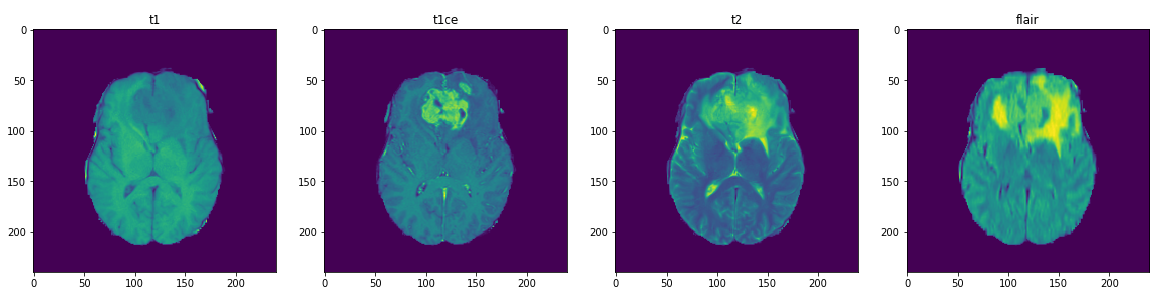
\includegraphics[scale=0.365]{images/title/0.png} \\
	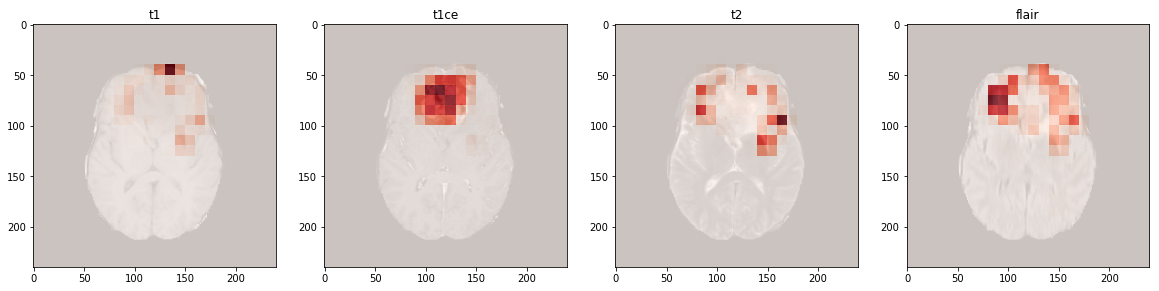
\includegraphics[scale=0.365]{images/title/5.png}
\end{textblock}

\begin{textblock}{154}(28,135)
	\begin{picture}(150,2)
		\put(0,0){\color{bfhgrey}\rule{150mm}{2mm}}
	\end{picture}
\end{textblock}
\color{black}

% Institution / titel / subtitel / authors / experts:
%---------------------------------------------------------------------------
\begin{flushleft}

\vspace*{115mm}

\fontsize{26pt}{28pt}\selectfont 
\heading				\\							% Read heading from file leader/title.tex
\vspace{2mm}

%\fontsize{16pt}{20pt}\selectfont\vspace{0.3em}
%Place your subheading here 			\\				% Insert subheading
\vspace{5mm}

\fontsize{10pt}{12pt}\selectfont
\textbf{TODO build a neural network for brain tumor segmentation, analize it with LIME and other methods} \\		% Insert text
\vspace{3mm}

% Abstract (eingeben):
%---------------------------------------------------------------------------
\begin{textblock}{150}(28,190)
\fontsize{10pt}{12pt}\selectfont
TODO: rework text
In this thesis work the objective is to develop a software suite enabling advance interpretability of machine learning (ML) approaches. The software suite builds on recent developments to visualize and harness explicability of complex machine learning systems, namely, occlusion tests during training of an ML model, L.I.M.E Ribeiro et al., and visualization tools from Zeiler et al. 2013.
 
As part of the thesis, a machine learning model for the BraTS dataset (benchmarking of Brain Tumor Segmentation) will be built. The algorithms described above (L.I.M.E, visualization tools) will then be used to inspect and evaluate how much these techniques help when building, optimizing and especially interpreting such a model in the medical imaging field.


\end{textblock}

\begin{textblock}{150}(28,225)
\fontsize{10pt}{17pt}\selectfont
\begin{tabbing}
xxxxxxxxxxxxxxx\=xxxxxxxxxxxxxxxxxxxxxxxxxxxxxxxxxxxxxxxxxxxxxxx \kill
Degree course:	\>      Bachelor of Science in Computer Science	\\		% insert name of degree course
Authors:		\> Fabio Anderegg		\\					% insert names
Tutor:	\> Peter von Niederhäusern		\\							% insert names
Constituent:	\> Mauricio Reyes, University of Bern					\\							% insert names
Experts:		\> Andreas Spichiger				\\							% insert names
Date:			\> \versiondate					\\							% read from file leader/version.tex
\end{tabbing}

\end{textblock}
\end{flushleft}

\begin{textblock}{150}(28,280)
\noindent 
\color{bfhgrey}\fontsize{9pt}{10pt}\selectfont
Berner Fachhochschule | Haute \'ecole sp\'ecialis\'ee bernoise | Bern University of Applied Sciences
\color{black}\selectfont
\end{textblock}


\end{titlepage}

%
% ===========================================================================
% EOF
%
		% activate for frontpage with picture
%% Control of versions :
% -----------------------------------------------

\begin{textblock}{180}(15,150)
\color{black}
\begin{huge}
Versions
\end{huge}
\vspace{10mm}

\fontsize{10pt}{18pt}\selectfont
\begin{tabbing}
xxxxxxxxxxx\=xxxxxxxxxxxxxxx\=xxxxxxxxxxxxxx\=xxxxxxxxxxxxxxxxxxxxxxxxxxxxxxxxxxxxxxxxxxxxxxx \kill
Version	\> Date	\> Status			\> Remarks		\\
0.1	\> 01.08.2013	\> Draft		\> Lorem ipsum dolor sit amet	\\	
0.2	\> 21.08.2013	\> Draft		\> Phasellus scelerisque	\\ 
0.3	\> 02.09.2013	\> Draft		\> Donec eget aliquam urna. Lorem ipsum dolor sit amet	\\ 
1.0	\> 26.01.2014	\> Final		\> Lorem ipsum dolor sit ametPhasellus scelerisque, leo sed iaculis ornare 	\\ 
1.1	\> 31.01.2014	\> Correction	\> Layout changed	\\
1.2	\> 07.02.2014	\> Addition		\> Chapter 1.1 extended	\\
\end{tabbing}

\end{textblock}

%\cleardoubleemptypage
\setcounter{page}{1}
\cleardoublepage
\phantomsection 
\addcontentsline{toc}{chapter}{Management Summary}
\chapter*{Abstract}
\label{chap:managementSummary}

Machine learning (ML) systems are achieving remarkable performances at the cost of increased complexity. Hence, they become less interpretable, which may cause distrust. As these systems are pervasively being introduced to critical domains, such as medical image computing and computer assisted intervention (MICCAI), it becomes imperative to develop methodologies to explain their predictions. Such methodologies would help physicians to decide whether they should follow/trust a prediction or not. Additionally, it could facilitate the deployment of such systems, from a legal perspective. Ultimately, interpretability is closely related with AI safety in healthcare.

Interpretability methods for (image) classification tasks are already well established. LIME, RISE, Grad-CAM and other methods deliver deep insights how a (convolutional) neural network came to its conclusion. Interpretability methods for image segmentation tasks in comparison are almost non-existent. The goal of this thesis is to modify an existing algorithm for classification to also work for segmentation or come up with a new method.

As part of the thesis, a machine learning model for the BraTS dataset (benchmarking of Brain Tumor Segmentation) has been trained. This model has been used to asses the newly developed methods.

Two methods have been successfully implemented: The existing method RISE (Vitali Petsiuk et. al.) has been modified to work on image segmentation tasks. In addition, an new method named Hausdorff Distance Mask has been developed. In essence, it works similar to to the Occlusion method propsed by Zeiler et. al. by occluding parts of the image and then comparing the network output to the baseline output from the unmodified original image. A visualization technique to generate a intuitivly understandable graphic for interpretation is also proposed.
\cleardoubleemptypage
%---------------------------------------------------------------------------

% Table of contents
%---------------------------------------------------------------------------
\tableofcontents
\cleardoublepage
%---------------------------------------------------------------------------

% Main part:
%---------------------------------------------------------------------------
\pagenumbering{arabic}

\chapter{Introduction}
Lime \cite{ribeiro2016should}
Some introduction text.
Some new introduction text.
\chapter{Introduction}
Modern machine learning models based on deep neural networks are achieving remarkable performance in many fields, including medical image analysis. In comparison with classic machine learning technologies like decision trees, it is much harder to explain how these neural networks came to their conclusions, because they use thousands to millions of training parameters.

In recent years, many methods for the interpretability of deep (convolutional) neural networks have been proposed, e.g. LIME \cite{ribeiro2016should}, RISE \cite{Petsiuk2018rise}, Grad-CAM \cite{selvaraju2017grad} or DeepLIFT \cite{shrikumar2017learning}.

\begin{figure}[h]
\centering
\caption{Examples of some interpretability methods for image classification \cite{visualattribution}}
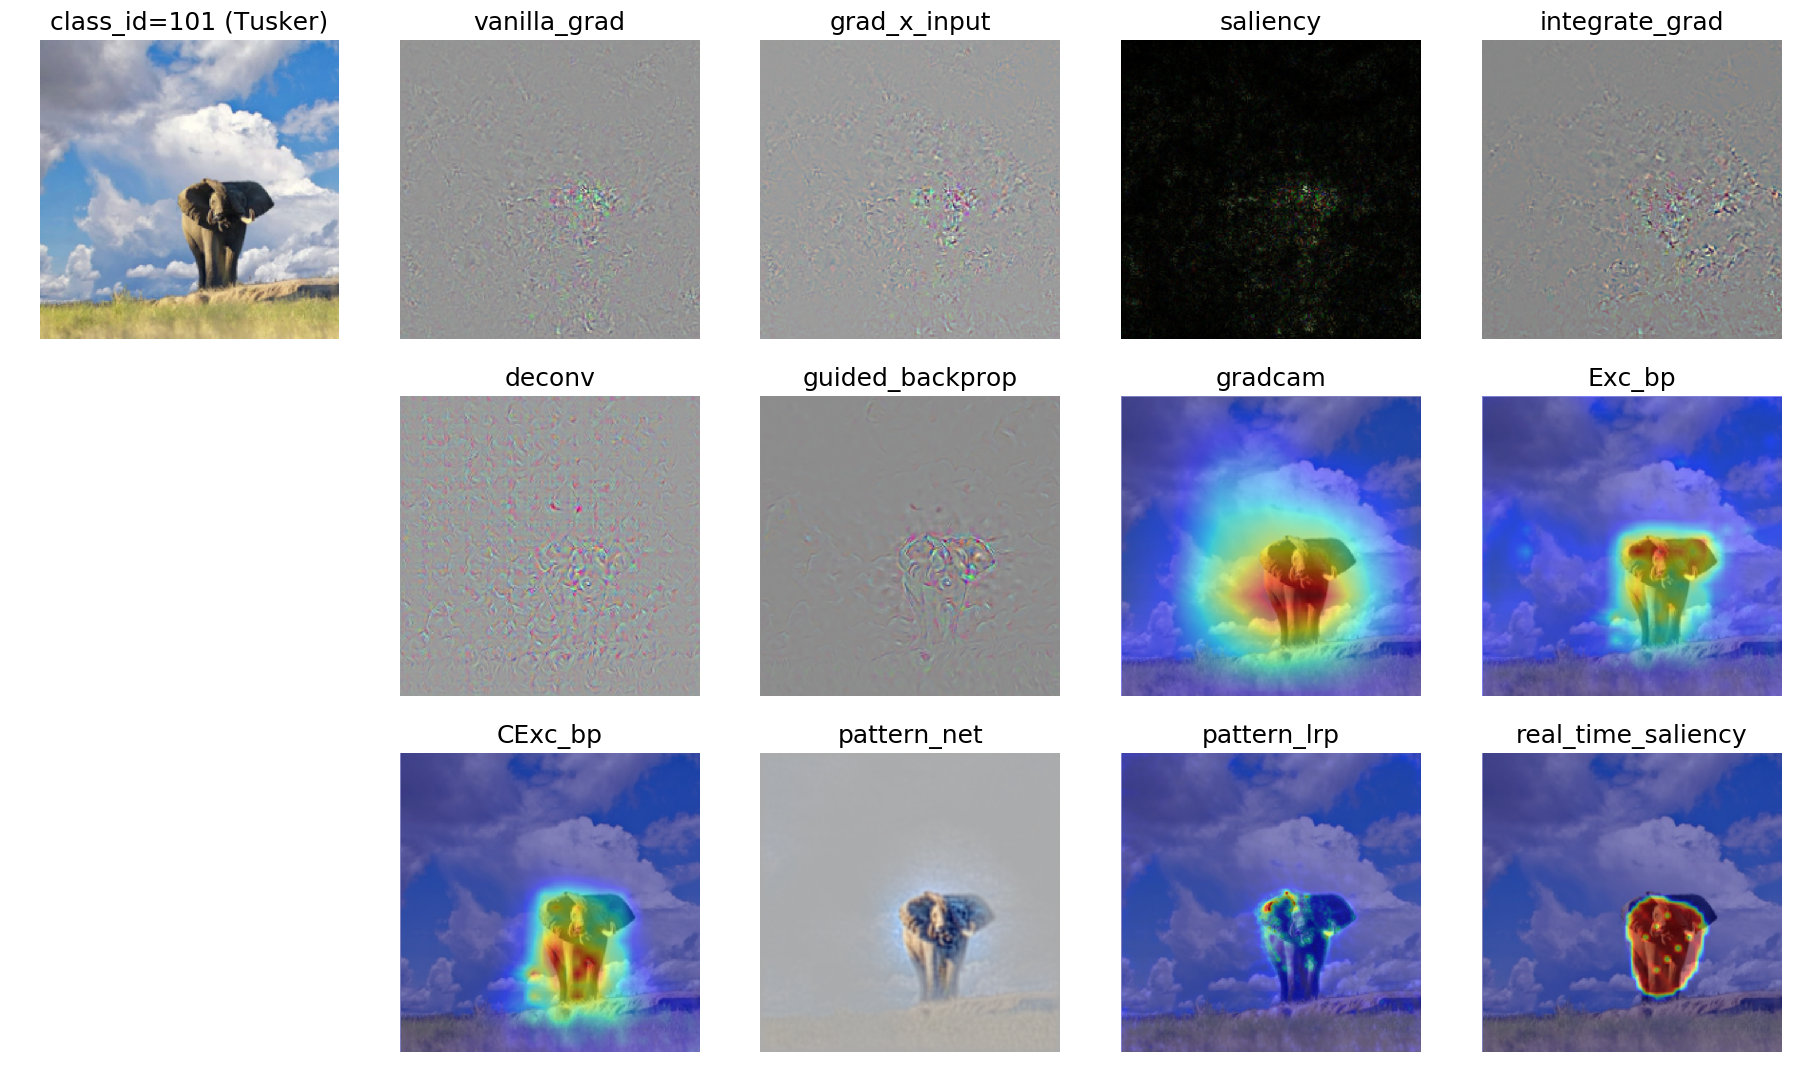
\includegraphics[width=14cm]{images/tusker_saliency.png}
\end{figure}

These methods focus on providing explanations and interpretability of classification problems for datasets like ImageNet \cite{imagenet_cvpr09} or MNIST \cite{lecun-mnisthandwrittendigit-2010}. Classification means that an algorithm can tell what is displayed on an image. ImageNet for example contains over 21,000 categories and 14 million images.

What has not yet been researched much is the interpretability of image segmentation tasks. With image segmentation, an algorithm does not only detect objects in images, but also marks (segments) where it found the specific object(s) in the image. On many image segmentation tasks, interpretability based on image regions like Grad-CAM (see image above) do not make that much sense, because the segmentation itself already returns a region of an image.

\begin{figure}[H]
\centering
\caption{Image segmentation on MRI scans of the brain \cite{soltaninejad2017automated}}
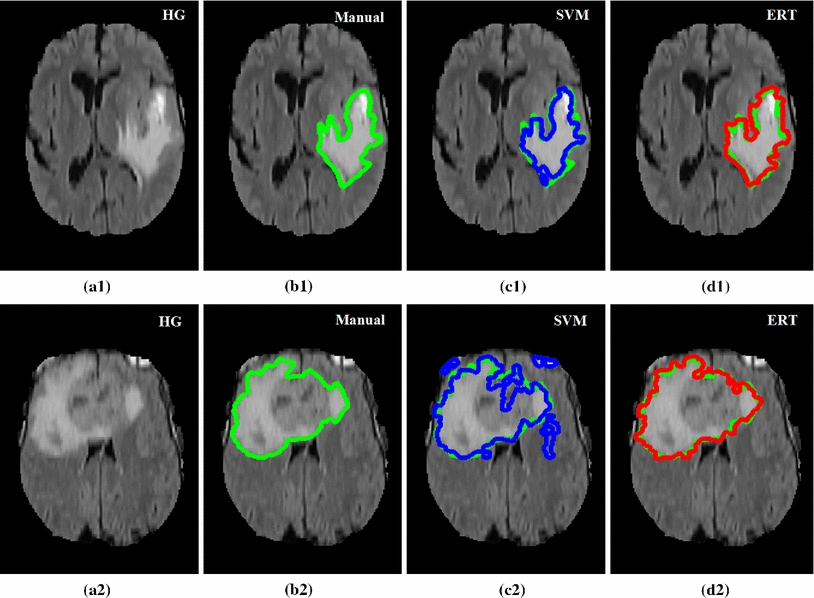
\includegraphics[width=10cm]{images/brain_segmentation.jpg}
\end{figure}

On other problems like finding and segmenting brain tumors on MRI images, medical professionals do not only look at the exact region where a tumor resides, but also at other regions of the brain. On the upper row of the scan above it is clearly visible that the tumor on the right side is extending the space used for the right half of the brain, and therefore many brain features are not symmetrical any longer. A neural network trained on this task should also use these cues to correctly segment the tumors. 

The goal of this thesis is to provide such a tool by modifying existing interpretability methods for classification tasks to work on image segmentation tasks. The tool generates images with marked regions similar to the ones in Figure 1.1. The marked regions represent the regions where the neural network took cues to generate the image segments as seen in Figure 1.2.

The customer for this thesis is Mauricio Reyes from the Institute for Surgical Technology and Biomechanics (ISTB) of the University of Bern. He and his team work in the medical imaging field together with the Inselspital Bern. One of the bigger projects is building a method to automatically segment brain tumors. The work of this thesis will help the team to understand what their machine learning model is doing and increase the trust of medical professionals into the methods because they can understand what the machine learning model is doing.

\chapter{Project planning overview}

The high-level approach for this thesis is:
\begin{itemize}
    \item Talk with the customer (Mauricio Reyes) to find out what his expectations are
    \item Use the current machine learning methods for interpretability on a simple classification task to learn what methods are available, how they work and and how they can be applied
    \item Train a neural network for brain tumor segmentation. This provides a real-world test bed for our further work
    \item Modify existing interpretability methods so they work on image segmentation tasks
    \item Provide a reusable Python library so other users can easily apply our developed methods
\end{itemize}

The author of this thesis is a part-time student normally working 60\% for a company. For this thesis he took a 6 week unpaid leave to work full-time on it.
Therefore a big part of the thesis should be completed in this 6 weeks. The 6 weeks start in the second week of the thesis.

In this 6 weeks, the main focus is writing the code to accomplish the defined goals in this document. The rest of the time will be used to finish the thesis document, package up the built program so it can easily be used by other people and complete all the other tasks required for the thesis (poster, movie, presentation, defense preparation etc.).

In the first 6 weeks the author plans to meet with the tutor (Peter von Niederhäusern) and the customer (Mauricio Reyes) each week to report on project progress and to get input on the thesis.
After the first six weeks, biweekly meetings are planned.

At least two meetings with the expert Andreas Spichiger will be scheduled.

For detailed time planning information, please consult the Gantt chart at the end of this document.

\chapter{Goals and requirements}

\section{Overview}
The resulting interpretability toolkit for image segmentation tasks takes the form of a Python library. The library should provide an easy to use interface for researchers to apply
the modified methods on their own neural network models and datasets.

\section{Functional requirements}
\subsection{Required goals}

\subsubsection{Build classification model and apply methods}
As a first step, a neural network should be trained on an image classification task in the medical imaging field.
After that, the existing interpretability methods RISE, LIME and Grad-CAM are applied on the trained model.
The goal of this step is to learn how these methods work, how they are applied and how their output looks like.

\subsubsection{Image segmentation model training}
To have a real world test bed to apply the newly developed methods, a neural network for image segmentation is trained.
The dataset used for this network is BraTS 2018, a dataset containing MRI scans of human brains which contain tumors.
The trained neural network should have an acceptable accuracy to generate meaningful output from the applied methods, but
does not have to be on the same level as current state of the art models. 

\subsubsection{Modify methods}
The main goal of the thesis is to modify the methods RISE and Grad-CAM to work on image segmentation tasks.
The two methods were chosen because they provide very good results, are widely used and there exist multiple high
quality implementations.

RISE is a black box method, which means it does not need to have access to the neural network itself,
just to the input images and the output of the network.

Grad-CAM is a white box method. It needs access to some of the layers of the neural network. The implication of this
is that applying the method requires configuration for a specific network architecture.

How these two methods can be modified to work on image segmentation instead of classification is currently unclear and therefore the main research topic of this thesis.

\subsubsection{Library and documentation}
To make the modified methods from above available to other researchers, a Python library will be built. Ideally, a library user can call a single function
which generates the desired output. Documentation of the provided functionality has to be written and examples how to use the library should be made available. The library should also be published on PyPI and Anaconda forge for easy installation by the standard package managers in the
Python and machine learning community.

\subsection{Optional goals}
The methods modified above (RISE and Grad-CAM) are black box and white box methods, respectively.
If a way is found how to modify these two methods to work with image segmentation tasks, it should be possible to modify other
methods in the same class (black/white box) in a similar way. These other methods will be chosen based on quality of output and availability and quality of existing implementations.

These methods will also be added to the Python library.

\section{System requirements}
The system requirements for the resulting Python library are:

\begin{itemize}
    \item Works with the PyTorch machine learning library
    \item Supports commonly used neural network architectures ResNet and densenet out of the box
    \item Supports other neural network architectures with minor modifications
    \item Does not depend on the underlying platform, only on a working Python installation with PyTorch
    \item Can optionally use Nvidia GPUs to speed up computation, but must also work on CPUs (with potentially greatly reduced performance)
    \item Can be installed with standard Python package managers (pip and Anaconda)
\end{itemize}

\section{Domain requirements}
The work in this thesis is done in the medical imaging field, because the customer comes from this field and because the problems in the field can benefit from the
work done in this thesis. The resulting Python library from this thesis will not be specific to the medical imaging field and should be applicable on all image segmentation tasks which take cues from parts of the image which are not contained in the resulting segmentation region.

\chapter{Detailed project plan}
\section{NIH Chest X-ray}
To get a general overview how the different interpretability methods work, we plan to build a model for a medical imaging task and apply some of the more commonly used methods on it. We will also search for existing pretrained models to complete this work faster and/or to have a more accurate model. The model will reuse an existing convolutional neural network architecture, e.g. ResNet or Inception.

The dataset selected for this task is the NIH Chest X-ray dataset \cite{wang2017chestx}. It contains 120,000 grayscale x-ray scans of chests and labels ranging from no findings to one or more diagnoses.

After building the model, we evaluate some of the common methods on the trained models. We want to determine which methods are independent of the used network architecture (methods that view the model as a black box). We also want to find implementations of the methods written for PyTorch or alternatively estimate how easy the methods could be ported to PyTorch. The last step is to show how the output of the method looks like and (optionally) check with a medical professional which output they think would be most helpful for the interpretability of a method.

\section{Brain tumors}
To build the methods to interpret image segmentation tasks, we need a real world task. Brain tumor segmentation is an interesting problem in the medical image field. Segmenting brain tumors manually is a tedious process, because MRI machines generate many slices of the brain which then have to be looked at one by one. Automating the process with machine learning will give medical professionals more time to do other tasks and also gives them more confidence in their manual work when supported by an automated model.

To build a working machine learning model, some medical background is required. We will investigate what types of brain tumors exist, how they look like on a scan and what scanner types are available (e.g. MRI/PET/CT). We also investigate how a tumor looks like on a specific scanner type.

\section{The BraTS 2018 dataset}
The BraTS \cite{menze2015multimodal} dataset contains MRI scans of the human brain and segmentation labels for found tumors in the scans.
The scan is 3D, saved as horizontal 2D slices. Every slice has four different black/white channels, each with a different setting of the MRI scanner.
There are 4 different labels for every slice, representing 4 different sizes of a tumor.

The tasks for this step is to figure out the data format of the dataset and then load the dataset into memory. Displaying some slices will show if the data was loaded correctly. Next, we extract multiple slices per scanned brain. We only use slices which contain visible tumors. This way we have 2D images we can feed into the convolutional neural network used for image segmentation.

The next step is loading the labels of the data. As recommended by Alain Jungo of the University of Bern, we will merge the two innermost region labels into one label and discard the other two labels.

\section{Model for the BraTS dataset}
A widely used architecture for segmentation (especially in the medical imaging field) is the U-Net \cite{ronneberger2015u}.

\begin{figure}[H]
\centering
\caption{The U-Net architecture}
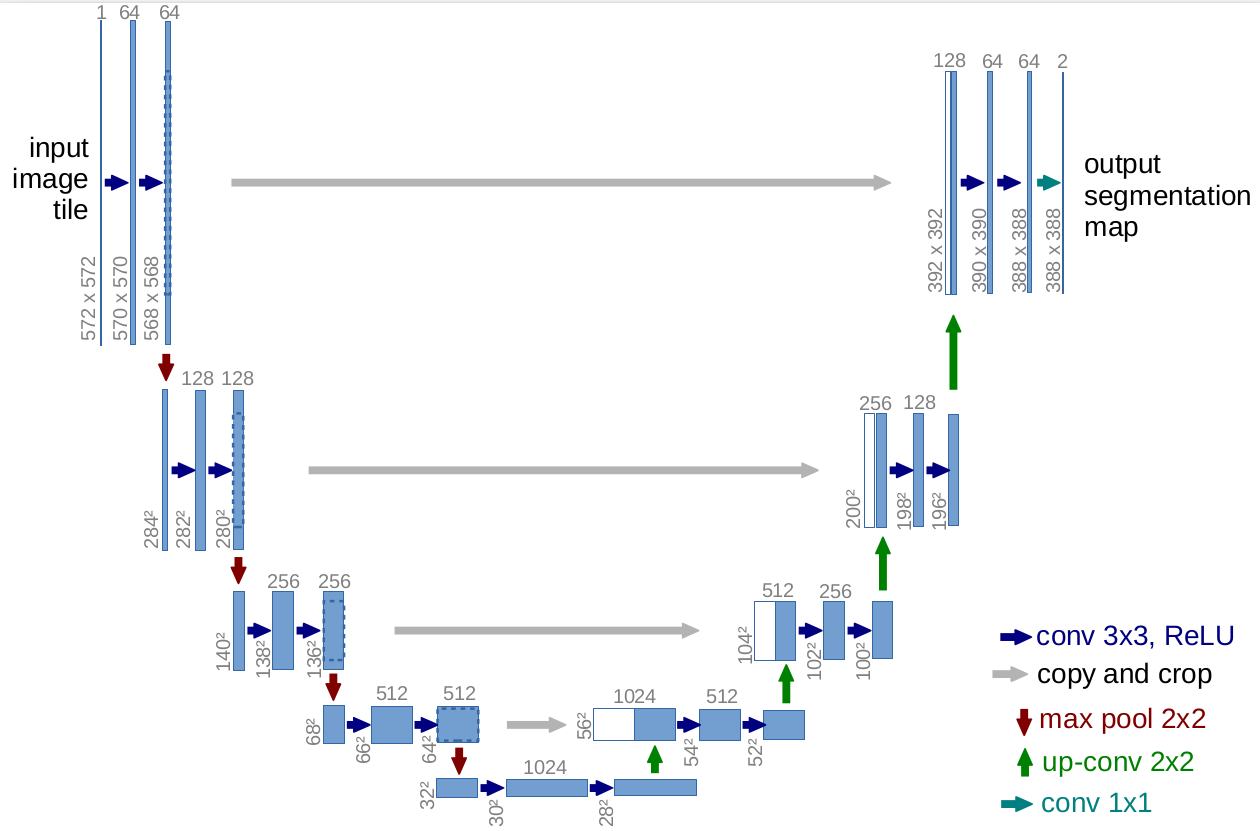
\includegraphics[width=10cm]{images/unet.png}
\end{figure}

The architecture uses a so called "encoder" network on the left side which generates features. A standard convolutional neural network can be used as an encoder. On the right side, instead of a linear layer mapping features generated from the convolutions to classes, a "decoder" network is used. The decoder network generates the output segmentation pixels based on the features extracted by the encoder.

We will build a U-Net using a standard convolutional neural network architecture. The fast.ai library contains a dynamic U-Net Python class which can automatically generate the decoder part of a U-Net by analyzing the CNN. We will evaluate if this works good enough or if a custom architecture is required.

\section{RISE method}
Randomized Input Sampling for Explanations (RISE) is a interpretability method that uses the model as a black box. It does not need to know anything about the underlying machine learning model, it only needs access to the input image and the probabilities of the output classes.

RISE generates a series of masks which get applied to the input image. The modified image is then run through the model and the changed probabilities of the output classes are recorded. From the probabilities of the different masks, a heatmap is generated which shows which parts of the image influence the correct classification of the image the most.

To use RISE for image segmentation, we have to find a way to replace the class probabilities with the segmentation pixels. This is part of the main research work of this thesis.


\section{Grad-CAM method}
The Grad-CAM \cite{selvaraju2017grad} (Gradient-weighted Class Activation Mapping) is a white box method which uses the parameters of a learned model to output a heatmap for a specific image classified by the network.

Grad-CAM is a widely used method with many high quality implementations which also generated an easy to understand output which can be used by medical professionals.

As with RISE, Grad-CAM is built for image classification tasks. Because the encoder part of a U-Net is a standard convolutional neural network, it should be possible to apply Grad-CAM on this part of the U-Net. If and how this is possible is part of the main research topic of this thesis.


\section{Library}
If the modification of the methods do work with image segmentation tasks, it is planned to build a Python library which allows to easily apply the methods to other datasets by its users. The library should be usable on PyTorch models. Documenting the library (e.g. on readthedocs.io) is essential for potential users, as are examples how to use the library, which can be extracted from the thesis source code.

Also planned is to publish the library on PyPI and conda-forge, so researchers can install the library in their environments.

\section{Other black box model methods (optional)}
There are other black box methods (e.g. LIME \cite{ribeiro2016should}) which work similar to RISE. If a successful method is found to apply RISE to image segmentation tasks, modifying these other methods to also work for segmentation should not be a major problem.

Building a high quality solution with RISE has a higher priority than adding additional methods.

\section{Other white box model methods (optional)}
As described above, there are many white box model methods which can be applied to this problem. If we can find a solution how to apply Grad-CAM, using other methods like PatternNet \cite{kindermans2017learning} or Meaningful Perturbation \cite{fong2017interpretable}.

\chapter{Evaluation and testing}
\section{Model evaluation}
There are many metrics to decide if a neural network model returns good results or not.
The two used metrics in this thesis will be loss and ROC/AUROC.

The loss describes how sure a network is with a given answer. An answer can be accurate, but the network is very unsure about it. The loss is especially useful to see if a neural network is learning something when training it. The loss in a training session should decrease with time, even when the accuracy is still very bad.
Another insight the loss can give is if the neural network overfits, i.e memorizes the input data instead of finding patterns in the data. If the training loss is going down (the loss calculated on the data which is used for training) but the validation loss (loss calculated on data the network has never seen before, which is only used to test the network performance) is going up, the network is starting to overfit.

The other metric is the ROC (Receiver Operating Characteristic) curve and the associated value AUROC (Area Under the ROC curve). This metric combines the standard statistical values from a confusion matrix (true positive, false positive, false negative and false negative) in a meaningful way.

There may be additional metrics specific for image segmentation which will be used if they are considered helpful.

\section{Testing}
Automatic testing for this thesis is very challenging, because it is difficult to decide if a specific interpretability method returns correct data, even for a human.

It is therefore very important to do thorough manual testing by looking at many examples generated by the methods. Cross checking the generated results with medical professionals is also important, because the output could make sense from a computer scientist's view, but is very wrong from a medical standpoint.

For the resulting Python library, unit and integration tests will be written with the main purpose of avoiding regressions and breaking client code. Integration tests are also useful as examples for the end user.

\section{Code quality}
The code quality and the observing of coding conventions and code style guides will be enforced by standard software in the Python community, namely flake8 which adheres to the Python PEP8 code standards and additional rules.

\chapter{Project management}
    \section{Team}
    The author and developer of this thesis is Fabio Anderegg.
    
    \section{Stakeholders}
    The following other people are also involved in the project:
    
    \begin{tabular}{| p{4cm} | p{3.5cm} | p{8cm} |}
        \hline
        \textbf{Name} & \textbf{Institute} & \textbf{Description} \\ \hline
        Peter von Niederhäusern & Bern University of Applied Sciences & Tutor \\ \hline
        Mauricio Reyes & Unversität Bern & Customer of the thesis. Group head of the Medical Imaging group of the ISTB. \\ \hline
        Andreas Spichiger & Bern University of Applied Sciences & External expert for the thesis. \\ \hline
        Alain Jungo & University of Bern & PhD student of Mauricio Reyes which works on the BraTS dataset for brain tumor segmentation. Technical expert and potential user for this thesis. \\ \hline
    \end{tabular}

\chapter{Infrastructure and technology}
This work will use the PyTorch \cite{paszke2017automatic} deep learning library. Most newer machine learning papers are written with PyTorch, because it is considered easier to learn and more powerful than TensorFlow and Keras \cite{pytorchvstensorflow}.

Other machine learning libraries will be used on demand, for example:

\begin{tabular}{|p{3cm}|p{12.5cm}|}
    \hline
    \textbf{Library} & \textbf{Description} \\ \hline
    Scikit & Diverse kits of machine learning libraries \\ \hline
    Matplotlib & Library to generate graphs \\ \hline
    PIL/Pillow & Image manipulation library \\ \hline
    NumPy & Matrix manipulation library \\ \hline
    pandas & Dataframe library \\ \hline
    torchvision & PyTorch extension for computer vision problems. Contains models for common architectures and pretrained parameters for these networks. Also contains tools for data augmentation. \\ \hline
\end{tabular}

The development of the system will take place inside Jupyter notebooks. Jupyter notebooks allow a very fast test and development cycle. The notebook server will be running on a powerful desktop computer of the author which is exposed to the internet, so the computational power is always available independent of the work location.

In addition, the GPU servers from the Bern University of Applied Sciences (NVIDIA DGX-1, 4x Tesla V100) and from the ISTB of the University of Bern (Unknown number and type of GPUs) are available. Because the required time to setup the code and infrastructure to use these servers is quite high, the usage of these systems is optional and will only be done if the reduced time to train the neural network is worth the additional work effort.


\chapter{Appendix}
\section{Description of thesis as submitted}

Machine learning (ML) systems are achieving remarkable performances at the cost of increased complexity. Hence, they become less interpretable, which may cause distrust. As these systems are pervasively being introduced to critical domains, such as medical image computing and computer assisted intervention (MICCAI), it becomes imperative to develop methodologies to explain their predictions. Such methodologies would help physicians to decide whether they should follow/trust a prediction or not. Additionally, it could facilitate the deployment of such systems, from a legal perspective. Ultimately, interpretability is closely related with AI safety in healthcare.

In this thesis work the objective is to develop a software suite enabling advance interpretability of machine learning (ML) approaches. The software suite builds on recent developments to visualize and harness explicability of complex machine learning systems, namely, occlusion tests during training of an ML model, L.I.M.E Ribeiro et al. (\url{https://homes.cs.washington.edu/~marcotcr/blog/lime/}), and visualization tools from Zeiler et al. 2013 (\url{https://cs.nyu.edu/~fergus/papers/zeilerECCV2014.pdf} and Github at: \url{https://github.com/InFoCusp/tf\_cnnvis}).
 
As part of the thesis, a machine learning model for the BraTS dataset (benchmarking of Brain Tumor Segmentation) will be built. The algorithms described above (L.I.M.E, visualization tools) will then be used to inspect and evaluate how much these techniques help when building, optimizing and especially interpreting such a model in the medical imaging field.

\pagebreak
\section{Project planning Gantt chart}

The following Gantt chart shows the time planning for the thesis based on the goals and detail planning described above.
The green bar shows the 6 weeks where the author works full time on the thesis and where most of the programming work should be done.
The dark blue bars show the work packages as definied in the detailed project plan chapter.
The light blue charts represent optional goals, which also function as reserve time if another goal needs more time than anticipated.
The red circles represent important milestones of the project.

\begin{ganttchart}[
bar/.style={fill=bar},
vgrid,
hgrid,
milestone/.append style={anchor=east,xshift=-1pt,fill=milestone,shape=circle,draw=milestone,},
title height=1.0,
x unit=6mm,
y unit title=8mm,
y unit chart=8mm,
]{10}{25}
    \gantttitle{Calendar weeks 2019}{16} \\
    \gantttitlelist{10,...,25}{1} \\
    \ganttbar[bar/.append style={fill=fulltimebar}]{Full-time work on thesis}{10}{15} \ganttnewline

    \ganttbar{Train chest X-Ray model}{10}{11} \ganttnewline
    \ganttbar{Apply interpretability methods}{11}{11} \ganttnewline
    \ganttmilestone{Goals definied}{11} \ganttnewline
    \ganttbar{Neural network for brain tumor dataset}{12}{12} \ganttnewline
    
    \ganttbar{Modify RISE method}{13}{14} \ganttnewline
    \ganttbar{Modify Grad-CAM method}{14}{15} \ganttnewline
    
    \ganttbar[bar/.append style={fill=optionalbar}]{Additional black box methods}{16}{18} \ganttnewline
    \ganttbar[bar/.append style={fill=optionalbar}]{Additional white box methods}{16}{18} \ganttnewline
    \ganttbar{Build Python library}{19}{19} \ganttnewline
    
    \ganttbar{Finish thesis text}{20}{22} \ganttnewline

    \ganttmilestone{Draft thesis text done}{22} \ganttnewline
    \ganttbar{Presentation preparation}{23}{24} \ganttnewline
    \ganttmilestone{Deadline thesis text \& presentation}{24} \ganttnewline
    \ganttmilestone{Thesis defense}{25}
\end{ganttchart}
\chapter{NHS Chest X-ray}
To find out what outputs the different methods generate, we started with a simple classification task in the medical image field:

* chest x-ray
* multi label classification
* current state of the art networkj: inception  resetnet v2 (accurate + fast to train on single GPU)
* using learnings and code from project2
* slightly modified inception resnet v2 implementation (grayscale instead of color)
* did not work, convert to RGB and downscale images (offline, preprocess.ipynb)

%---------------------------------------------------------------------------

% Selbständigkeitserklärung
%---------------------------------------------------------------------------
\cleardoublepage
\phantomsection 
\addcontentsline{toc}{chapter}{Declaration of authorship}
\chapter*{Declaration of primary authorship}
\label{chap:declaration_authorship}

\vspace*{10mm} 

I hereby confirm that I have written this thesis independently and without using other sources and resources than those specified in the bibliography. All text passages which were not written by me are marked as quotations and provided with the exact indication of its origin.

\vspace{15mm}

\begin{tabbing}
xxxxxxxxxxxxxxxxxxxxxxxxxxxxxx\=xxxxxxxxxxxxxxxxxxxxxxxxxxxxxx\=xxxxxxxxxxxxxxxxxxxxxxxxxxxxxx\kill
Place, Date:		\> Bern, 05.03.2019 \\ \\ 
Last Name, First Name:	\> Anderegg Fabio	\\ \\ \\ \\ 
Signature:	\> ...................................... \\
\end{tabbing}

%---------------------------------------------------------------------------

% Glossary
%---------------------------------------------------------------------------
%\cleardoublepage
%\phantomsection 
%\addcontentsline{toc}{chapter}{Glossay}
%\renewcommand{\glossaryname}{Glossay}
%\printnomenclature
%---------------------------------------------------------------------------

% Bibliography
%---------------------------------------------------------------------------
\cleardoublepage
\phantomsection 
\addcontentsline{toc}{chapter}{Bibliography}
\bibliographystyle{IEEEtranS}
\bibliography{database/bibliography}{}
%---------------------------------------------------------------------------

% Listings
%---------------------------------------------------------------------------
\cleardoublepage
\phantomsection 
\addcontentsline{toc}{chapter}{List of figures}
\listoffigures
\cleardoublepage
\phantomsection 
\addcontentsline{toc}{chapter}{List fo tables}
\listoftables
%---------------------------------------------------------------------------

% Index
%---------------------------------------------------------------------------
\cleardoublepage
\phantomsection 
\addcontentsline{toc}{chapter}{Index}
\printindex
%---------------------------------------------------------------------------

% Attachment:
%---------------------------------------------------------------------------
\appendix
\settocdepth{section}
\chapter*{APPENDICES}
\addcontentsline{toc}{chapter}{APPENDICES}

\begingroup\let\clearpage\relax
\chapter{Code}
\label{chap:appendix_arb}
\endgroup

TODO: do we need that? link to github repo?
%\include{appendix/appendixexempleB}
%---------------------------------------------------------------------------

%---------------------------------------------------------------------------
\end{document}

